\section{Robust Verification of Quantum Computations}
\label{sec:ubqc}

\paragraph{Measurement Based Quantum Computation.}
An MBQC algorithm, also called \emph{measurement pattern}, consists of a graph $G = (V,E)$, two vertex sets $I$ and $O$ defining input and output vertices, a list of angles $\{\phi_v \}_{v \in V}$ with $\phi_v \in \Theta := \{k\pi/4\}_{0 \leq k \leq 7}$ and a function \(f:O^c\rightarrow I^c\) called \emph{flow}.

To run it, the client instructs the server to prepare the graph state $\ket{G}$: for each vertex in $V$, the server creates a qubit in the state $\ket{+}$ and performs a $\CZ$ gate for each pair of qubits in $E$. A canonical example of such a resource state is shown in Figure \ref{fig:graph}. The client then asks the server to measure each qubit of $V$ along the basis $\left\{\ket{+_{\phi'_v}}, \ket{-_{\phi'_v}}\right\}$ in the order defined by the flow of the computation, with $\ket{+_\alpha} = (\ket 0 + e^{i\alpha}\ket 1)/\sqrt 2$. The corrected angle $\phi'_v$ is given by $\phi'_v = (-1)^{s_v^X}\phi_v + s_v^Z\pi$ for binary values of $s_v^X$ and $s_v^Z$ that depend only on the outcomes of previously measured qubits and the flow---the interested reader is referred to~\cite{HEB04multiparty,DKP07measurement-calculus} for details about the flow.

As shown in \cite{DKP07measurement-calculus}, the MBQC model is equivalent to the circuit model, so that any \(\mathsf{BQP}\) algorithm in the circuit model can be translated in the MBQC model with at most polynomial overhead.

\begin{figure}[!h]
    \centering
    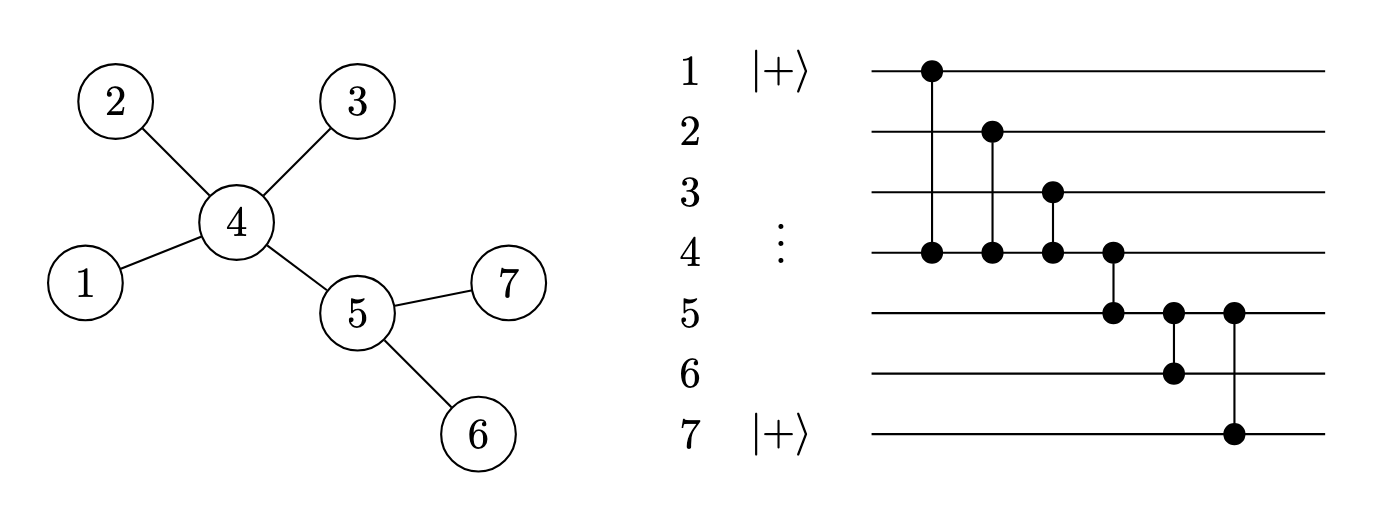
\includegraphics[width=0.5\linewidth]{graph.png}
    \caption{Translation of a graph state (left) into a circuit (right). Vertices correspond to qubits prepared in $\ket{+}$, and CZ gates between qubits correspond to vertices that share an edge in the graph.}
    \label{fig:graph}
\end{figure}

\paragraph{Hiding the Computation.}
In MBQC, a computation can be easily hidden if, instead of the server preparing each qubit, the client (i) for all $v \in V$ sends $\ket{+_{\theta_v}}$ with $\theta_v$ chosen uniformly at random in $\Theta$; (ii) asks the server to measure the qubits in the basis defined by the angle $\delta_v = \phi'_v + \theta_v + r_v\pi$ for $r_v$ a random bit, while keeping $\theta_v$ and $r_v$ hidden from the server; and (iii) uses $s_v = b_v \oplus r_v$ where $b_v$ is the measurement outcome to compute $s_v^X$ and $s_v^Z$ defined above. The random sampling of $\theta_v$ implements a One-Time Pad for $\phi'_v$ while $r_v$ does the same for the measurement outcomes. 

Indeed, this initial idea can be turned into a protocol that provides blindness even when the initial unencrypted qubits are not in the \(\ket +\) state. This is the Universal Blind Quantum Computing protocol introduced in~\cite{BFK09universal}.  It works by adding a random bit flip \(\X\) per qubit, updating the measured angles accordingly, and also one-time-padding the returned output.

\begin{protocol}[Universal Blind Quantum Computing (UBQC)]
  \label{proto:ubqc}
\item
  \begin{algorithmic}[0]
    \State \textbf{Public information}: A graph \(G\) and a flow \(f\).
    \State \textbf{Client's input}: \(\rho\) the initial state of the qubits at nodes of \(G\), a measurement pattern using the flow \(f\), that is a list of measurement angles \(\{\phi_{v}\}_{v\in V}\).

    \Procedure{State Encryption}{}
    \State For each \(v\in V\) sample the following encryption secrets  \(a_v \sample \{0,1\}\), \(r_v \sample \{0,1\}\), \(\theta_v \sample \Theta\).
    \State Apply \(\Z(\theta_{v}) \X^{a_{v}}\) to qubit at \(v\).
    \EndProcedure

    \Procedure{Graph State Creation}{}
    \State The server applies \(\CZ\) gates for all edges of $G$.
    \EndProcedure
    
    \Procedure{Encrypted Computation Orchestration}{}
    \State In the order of the flow, the client sends a measurement angle for qubit \(v\) as \(\delta_{v} = \phi_v' + \theta_v + r_v \pi\), and receives \(b_v\) from the server, corresponding to the encoded measurement outcome for this measurement. Here, \(\phi_v'\) is computed as above using \(s_u = b_u \oplus r_u\) as the decrypted measurement outcome for the measurement occurring at \(u\).
    \EndProcedure
  \end{algorithmic}
\end{protocol}

\paragraph{Generating Test Rounds}
\label{sec:test-rounds}
Given a graph \(G=(V,E)\), and a vertex \(v \in V\) such that \(v\) is prepared in \(\ket +\) and all its neighbors in \(G\) are prepared in \(\ket 0\), it is easy to verify that after the creation of the graph all these qubits remain unchanged. This is because a \(\CZ\) gate applied to a qubit in \(\ket 0\) leaves both untouched. If \(\X\) is then measured on \(v\), this would yield the +1 outcome. We call such preparation of \(v\) and neighbors a \emph{trap}, and the outcome of the \(\X\) measurement on \(v\) the \emph{trap outcome}; \emph{passed} if +1 and \emph{failed} if -1. 

Several traps can be inserted in a given round as long as they are not neighbors. Such a round is then called a \emph{test} round. For rVBQC to provide security, each vertex of \(G\) must be a trap in a constant fraction of the test rounds, as all traps cannot be placed in a single round. Indeed, for a \(k\)-colorable graph, \(k\) different types of test rounds are enough to fulfill this constraint. This gives the following routine:
\begin{routine}[Test Round Sampling]
  \label{routine:test-sampling}
  \item
  \begin{algorithmic}[0]
    \State A \(k\)-colorable graph \(G\) and a \(k\)-coloring \(\{V_i\}_i, \ \dot{\cup}_i V_i = V\)
    \Procedure{Test Round Sampling}{}
    \State \(i \sample [k]\)
    \State Output the preparation of traps at \(v \in V_i\)
    \State Output a measurement pattern so that all \(v \in V_i\) are measured with angle 0 corresponding to measuring \(\X\), setting the rest to random values in \(\Theta\).
    \EndProcedure
  \end{algorithmic}
\end{routine}



% \paragraph{Verifiability Through Trap Insertion.}
% Verifiable protocols allow the client to check that its computation has been done correctly.
% To do this, the client enlarges the graph used for the computation to insert traps.
% These traps are made from qubits randomly prepared in $\ket{+_{\theta}}$ states and disconnected from the sub-graph used for performing the desired computation with the help of \emph{dummy qubits} -- i.e.~randomly initialised qubits sent by the client in states $\{\ket{0}, \ket{1}\}$.
% The first verification protocol via trapification was introduced in~\cite{fk}.
% It was further optimised into the \emph{Verifiable Blind Quantum Computation Protocol} (or VBQC) of~\cite{KW15,XTH20}, achieving a linear overhead.

% \paragraph{Verifying the Computation.}
% Verification in the Compute and Test paradigm, verification is obtained by randomly interleaving computation rounds and test rounds. The latter are made from qubits randomly prepared in $\ket{+_{\theta}}$ states and disconnected from the rest of the graph-state used for performing the desired computation with the help of \emph{dummy qubits}---i.e.~randomly initialised qubits sent by the Client in states $\{\ket{0}, \ket{1}\}$. Because both types of rounds use the same underlying graph-state and flow, their nature can be hidden from the server using the UBQC protocol sketched previoulsy.

% This can be encapsulated in the following protocol:

% \begin{protocol}[Robust Verifiable Blind Quantum Computation (rVBQC)]
% \item
%   \begin{algorithmic}[0]
%     \State{\textbf{Client's Inputs:}} Angles $\qty{\phi_v}_{v \in V}$ and flow $f$ on graph $G$, classical input to the computation $x \in \bin^{\#I}$ (where $\#X$ is the size of $X$).

%     \State{\textbf{Protocol:}}
%     \begin{enumerate}
%     \item The Client chooses uniformly at random a partition $(C, T)$ of $[n]$ ($C \cap T = \emptyset$) with $\#C = d$, the sets of indices of the computation and test rounds respectively.
%     \item[2.] For $j \in [n]$, the Client and the Server perform the following sub-protocol (the Client may send message $\Redo_j$ to the Server before step 2.c while the Server may send it to the Client at any time, both parties then restart round $j$ with fresh randomness):
%       \begin{enumerate}

%       \item[(a)] If $j \in T$ (test), the Client chooses uniformly at random a colour $\mathsf{V}_j \in_R \qty{V_k}_{k \in [K]}$ (this is the set of traps for this test round).
%       \item[(b)] The Client sends $\#V$ qubits to the Server. If $j \in T$ and the destination qubit $v \notin \mathsf{V}_j$ is a non-trap qubit (therefore a dummy), then the Client chooses uniformly at random $d_v \in_R \bin$ and sends the state $\ket{d_v}$. Otherwise, the Client chooses at random $\theta_v \in_R \Theta$ and sends the state $\ket{+_{\theta_v}}$.
%       \item[(c)] The Server performs a $\CZ$ gate between all its qubits corresponding to an edge in the set $E$.
%       \item[(d)] For $v \in V$, the Client sends a measurement angle $\delta_v$, the Server measures the appropriate corresponding qubit in the $\delta_v$-basis, returning outcome $b_v$ to the Client. The angle $\delta_v$ is defined as follows:
%         \begin{itemize}
%         \item If $j \in C$ (computation), it is the same as in UBQC, computed using the flow and the computation angles $\qty{\phi_v}_{v \in V}$. For $v \in I$ (input qubit) the Client uses $\tilde{\theta}_v = \theta_v + x_v\pi$ in the computation of $\delta_v$.
%         \item If $j \in T$ (test): if $v \notin \mathsf{V}_j$ (dummy qubit), the Client chooses it uniformly at random from $\Theta$; if $v \in \mathsf{V}_j$ (trap qubit), it chooses uniformly at random $r_v \in_R \bin$ and sets $\delta_v = \theta_v + r_v\pi$.
%         \end{itemize}
%       \end{enumerate}

%     \item[3.] For all $j \in T$ (test round) and $v \in \mathsf{V}_j$ (traps), the Client verifies that $b_v = r_v \oplus d_v$, where $d_v = \bigoplus_{i \in N_{G}(v)} d_i$ is the sum over the values of neighbouring dummies of qubit $v$. Let $c_{\mathit{fail}}$ be the number of failed test rounds (where at least one trap qubit does not satisfy the relation above), if $c_{\mathit{fail}} \geq w$ then the Client aborts by sending message $\Abort$ to the Server.
      
%     \item[4.] Otherwise, let $y_j$ for $j \in C$ be the classical output of computation round $j$ (after corrections from measurement results). The Client checks whether there exists some output value $y$ such that $\# \left\{ y_j \, | \, j \in C,\, y_j = y \right\} > \frac{d}{2}$. If such a value $y$ exists (this is then the majority output), it sets it as its output and sends message $\Acc$ to the Server. Otherwise it sends message $\Abort$ to the Server.
%     \end{enumerate}
%   \end{algorithmic}
% \end{protocol}
